\chapter{Introduction}\label{chap:intro}

Knowledge Discovery in databases is currently the fastest
growing area of computing research \cite{knowdisc91}, not least because it can be said
to be the hybrid of a number of other research disciplines as shown in
figure~\ref{fig:dm_process}, primarily statistics, machine learning,
and database theory, yet with direct real-world application.

\medskip

In this thesis we propose a number of approaches to different
knowledge discovery
problems in databases which contain indefinite or temporal
information. Throughout we use Numerical Depdencies (NDs), a
generalisation of the FD, and 
show how they are suitable in numerous ways.  We also use and develop some
resampling processes, computationally intensive statistical
procedures, which are well suited to inferring information from
databases containing temporal and indefinite information. 


\begin{figure}
\centerline{\scalebox{0.5}{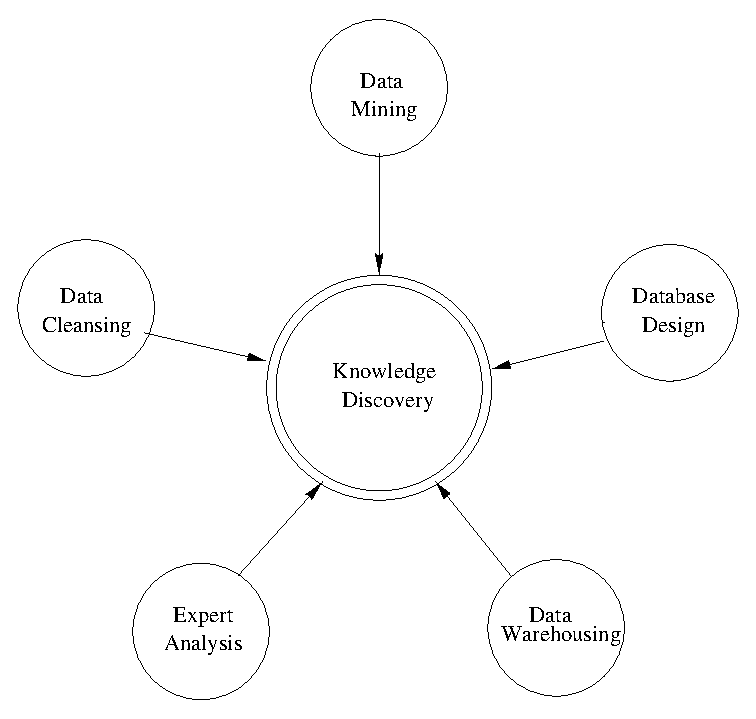
\includegraphics{../literature/kdd_component.eps}}}
\caption{\label{fig:kdd_component}Components of the
         Knowledgy Discovery Process}
\end{figure}

\section{The Hypothesis}
\index{hypothesis}

In this thesis we propose that data mining can be achieved using NDs,
particularly in many temporal databases or databases containing
indefinite information. Moreoever, the application of NDs allow data
mining principles to be exercied on categorical data, often the bulk
of many corporate databases, or a combination of categorical and
numerical data.

\section{Knowledge Discovery in Databases and this thesis}
			\index{Knowledge Discovery!Goals}
			\index{Knowledge Discovery!Outline}
			\index{Machine Learning!and Data Mining}
			\index{Pattern Discovery}
			\index{Data Warehouse}

 
\begin{figure}
\centerline{\scalebox{0.5}{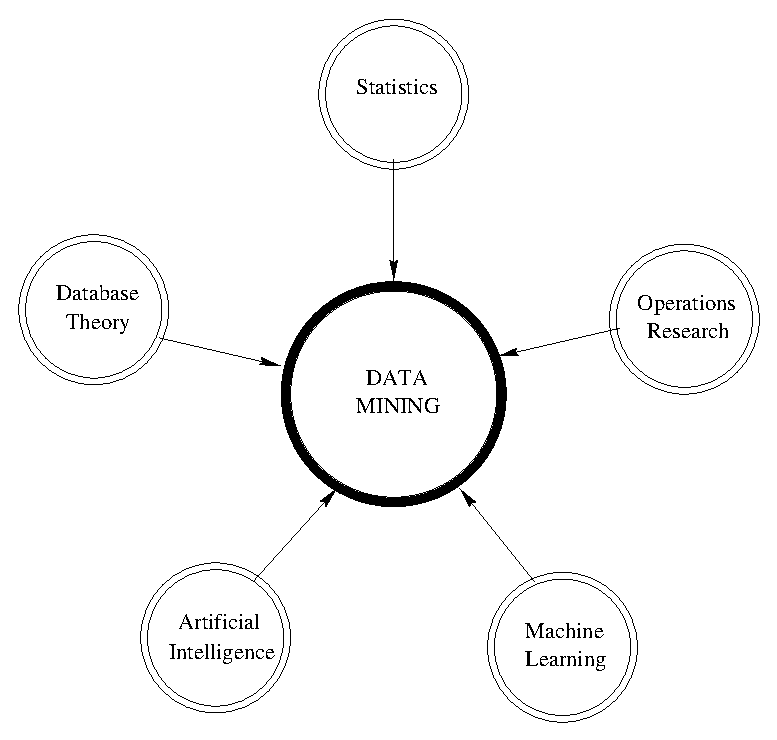
\includegraphics{../literature/dm_process.eps}}}
\caption{\label{fig:dm_process}Components of the Data
Mining Process}
\end{figure}
  
 
\begin{figure}
\centerline{\scalebox{0.5}{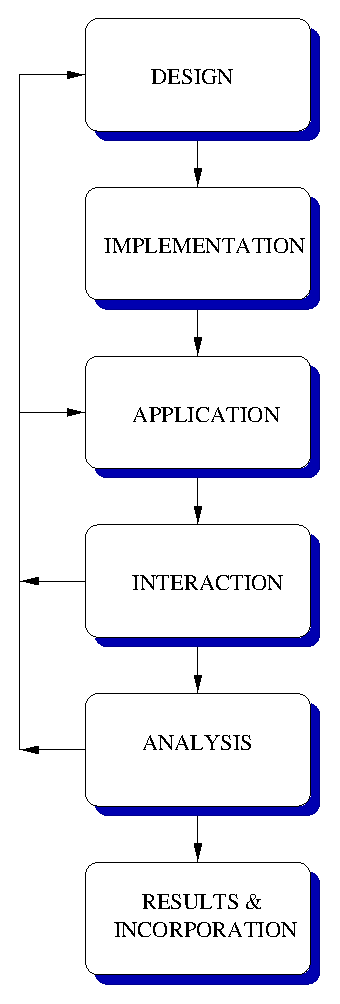
\includegraphics{../literature/kd_process.eps}}}
\caption{\label{fig:kd_process}The Knowledge Discovery
Application Cycle}
\end{figure}

The following widely accepted definition is due to \cite{kdd96}:

\begin{definition}[Knowledge Discovery in Databases]
\begin{rm} Knowledge Discovery in Databases is defined as {\em the nontrivial extraction of implicit, previously unknown, and potentially useful information from a database}.   
\end{rm}
\end{definition}

Knowledge Discovery may only provide {\em potentially} useful
information given that it may frequently discover relations, possibly
weak, between unconnected real-world information or even relations
that do not serve the interests of the user.  This includes the
possible discovery of redundant information. For instance, in a
medical database a system may discover a dependency $pregnant
\rightarrow female$; obviously such information is trivial.  Methods
to prevent such redundant information generation may include the
specification of trivial associations before the mining process takes
place and continuous interaction with an expert, a much understated
component of knowledge discovery, defined as {\em data
archaeology} as well as provision of a dependency template upon which
knowledge is discovered. The definition above may be extended by the restriction
that all useful information is also {\em understandable} by the users
of the data mining system. 

\medskip
In the sequel we make injudicious use of terms such as {\em data
mining}, {\em data mining algorithms}, {\em data mining
procedures/processes}. These terms can be said to refer to the general
process of data mining. 

\medskip

Data mining is a part of the larger process of knowledge discovery, as
figure~\ref{fig:kdd_component} shows. Recent work has included
research into formalising the data warehouse \cite{hgmw95,inm96a}, the canvas for
the application of data mining, and there has been significant
data cleansing research.  Knowledge
discovery refers to the process of extracting patterns and relationships 
from the data whereas data mining refers to the actual process of applying
these algorithms to the data, though many of the boundaries are vague.
In data mining applications a key step is 
the preparation of data for analysis, in figure~\ref{fig:kd_process},
an example of a KDD application cycle, we assume that the
design and application sections handle any required data
cleaning. Many data mining algorithms may also divide the data into suitable training and validation data.

KDD encompasses a number of different
technical approaches, such as clustering, data summarization, learning
classification rules, finding dependency networks, analyzing changes,
and detecting anomalies.  
KDD is seen as a research frontier for both database research and
machine learning as well as the 
possible inclusion of many other AI based techniques such as Natural Language 
Processing and Distributed AI methods \cite{kdd96}.  Since database 
technology has already found  
wide application in many fields, machine learning research obviously
stands to gain from this greater exposure and established
technological foundation. \cite{xiao95} characterises learning from a
database as a triple $\langle$ D, C, A $\rangle$ where 
D is the data, C the concept biases, and A the language in which to
phrase the definitions. He also notes that as a database stores no  
negative information induction should be performed cautiously to avoid
over generalisation.

\medskip

Temporal Knowledge Discovery relates to forecasting events in the future and for analysing
patterns which occur over time. Nearly all databases in use contain a
temporal component and there has been much data mining work on
temporal knowledge discovery \cite{alss95,pt96,bc96,bt98}. Temporal
Databases have been a significant area of research in the last few
years \cite{tcg93,ct95}, unsurprising given the need for temporal
support in numerous applicatons, particularly in the financial and
medical domains. Building on this work is the rapid rise of, and need
for, temporal data mining applications.  

\medskip

Additionally database now have a need for the representation of
indefinite information, required in database which may have design or
scheduling applications, and thereby providing the facility to
represent disjunction in cells \cite{il84,inv91,ivv95,vn95}.  Perhaps
given that there has not yet been widescale deployment of database
applications allowing indefinite information there has consequently
been minimal research on the data mining of relations containing
indefinite information \cite{cl98b}.

\medskip

Data mining and statistics have been substantially analysed
\cite{fhs96,gmp97}. Data reduction is a common step before statistical
analysis. Many data mining algorithms seek to make inferences from
sample data; classical statistics refers to this as {\em estimation}
and our work incorporates resampling processes \cite{efro79,et86,et93}
to achieve this. One of the prime goals of numerous data mining
methodologies is prediction and this is inherently related to the
representation of temporal data and the area of statistics known as
{\em Time Series Analysis}. Time Series Analysis when applied in a
 database is used for:

\begin{enumerate}
\item Identifying workers in different categories 
\item Identifying demand and modify supply accordingly
\item Calculate the patterns and changes in salary changes over time
\item Calculate the expense of projects over different time periods
\end{enumerate}

The Classic multiplicative models views time series as containing four
components, namely trend, cycles, seasonal and irregular patterns.
Trends may be up or down and can be used to characterise the time
series over a long time irrespective of short term fluctuations.
Cycles display a recurring up and down movement around trend levels,
including expansion and contraction. Seasonal patterns complete within
a given time period. Finally, irregular patterns account for erratic
changes in a time series and may be modelled as noise in the data.
\smallskip

The above may be understood using many techniques including trend moving averages, ratio-to-moving averages (for deriving
the seasonal component), difference equations for model
representation. Using these time series may be extrapolated.
Related issues are (1) Granularity Changes (2) Application of Moving
windows, and (3) Attribute value transformation. The temporal logic we
present, as well as the related work we survey
\cite{frm94,lai93,alss95,dgm97,dlm98}, is closely linked with many
aspects of (stationary) Time Series Analysis. \cite{gmp97} also
tackles the issues of how data mining is extending and not simply
repeating previous statistical research. There have been significant
use of data mining algorithms which have much need for statistical
functions, not least in the scientific domain on applications as
diverse as astronomical cataloguing through to geological sensing for
earthquake detection \cite{fhs96}.

\medskip

Recently there have been a number of different approaches to temporal
data mining, much stemming from machine learning work on pattern
matching \cite{lai93,alss95}. There seems to be a demarcation between research based on
data mining from temporal databases and research using time series as
the input data set from which knowledge is to be discovered. Our
approach allows for discovery from either or a combination of the
two. Within the limits of our experience this is a new basis for data
mining though we are not stating that other methodologies could not be
adapted for such purposes.

\medskip

There have been many recent calls for a data mining SQL to be formally
defined \cite{im96}. It is interesting to note that discovery in this
sense is closely linked to the power of the query language. Similarly,
we may view rule discovery using temporal logic directly dependent on
the expressiveness of the logic.

\medskip

Temporal Logic is used for temporal data mining in
\cite{pt96,bt98}. It has been shown to be sufficient for expressing
temporal relationships that have been discovered. We choose not to
apply this logic directly but instead develop a logic with statistical
functionality so that we do not have to present {\em confidence} and
{\em frequency} values for the rules that we discovery (akin to work
on association rules \cite{ais93,kmrtv94,hkmt95}) as the rule discovery
itself is representative of specific statistical values embedded in
the logic. Our work on temporal relations is pattern focused; we do
not attempt to discover a global model, the undoing of many time
series analysis studies, but logical rules which describe local rules
on subsequences of the temporal data set. Of course these can be, if
desired, extended to global conditions.


\subsubsection{Data Mining: Achievements and Goals}\label{subsec:goals}
\index{Data Mining!Algorithm}
\index{Data Mining!Introduction}
\index{Catalytic Relation}

\section{Main Results and Contribution}
\index{Contribution}


This thesis makes the following contributions:
\begin{enumerate}
\item Numerical Dependencies (NDs) are shown to be efficient and useful for 
data mining in that they provide a clear notion of proximity to FDs.
NDs are shown to be able to efficiently and accurately approximate FDs
in a relation with an easily understood semantics. 
An evolutionary database design procedure is introduced as a 
motivation for real-world ND applications as a precursor to their application
in non-standard database domains. The lattice properties of NDs are
exploited to provide a metric for data mining which we use in this work. 
\item We provide a detailed study on an approach which uses NDs to
provide approximations to the Consistency Problem, namely the
NP-Complete problem of finding a definite world that satisfies a set
of FDs within a relation containing indefinite data. 
\item Procedures for applying the Bootstrap within relations containing
indefinite and temporal data are defined and shown to be useful via extensive
simulations. They include a dynamic procedure for application of the
boostrap in indefinite relations for sample size determination. 
\item A Temporal logic for NDs is presented. This logic is then used
for mining sequences of relations. We examine the sequences for proximity
to functional FD set satisfaction as well as considering the evolution
of {\em ideal} AS and comparing this to a standard Time Series
Analysis. The logic is transferable to standard time series and other
linearly ordered sequences.
\item We present a model for the application of our temporal data
mining system to a sequence of temporal relations.
\item The thesis also presents a taxonomy of standard and temporal 
dependency data mining, 
placing our work in context, as well as making suggestions for future research.
\end{enumerate}




\section{Outline of the Thesis}
\index{Thesis Outline}

After this introduction, Chapter~\ref{chap:review} formally presents
the required relational database theory so that the remainder of the
work is self-contained.  All of the relevant theory presented is
placed in the context of this research and related work. Additionally,
we present related data mining research, focusing on three areas. (1)
We examine functional dependency data mining and the methods used to
find approximations to FDs \cite{km95,at94,Mann92,sf93,HS95,pk95,bel95b,psm93}, of which using NDs is part of our
contribution, shown in Chapter~\ref{chap:numdep}. (2) We briefly examine work conducted on mining of
indefinite information, related to our study of the consistency
problem, and (3) temporal data mining research is discussed so that
the reader is able to appreciate the contribution of the
work in chapters~\ref{chap:templog}
and~\ref{chap:tempresult}. Chapter~\ref{chap:review} concludes with a
brief presentation of
resampling in statistical applications, which is then expanded upon in
Chapters~\ref{chap:consistency} and~\ref{chap:tempresult}.

\medskip

Chapter~\ref{chap:numdep} presents ND theory with regard to data
mining, including a chase procedure for NDs. We show how a
{\em data mining} evaluation function is used for assessment, related
to approximation work presented in
chapter~\ref{chap:review}. Additionally, research on applying NDs for
mining within relations is discussed and compared with other
approaches. We also present a practical database design tool for randomly
evolving example relations which satisfy FD sets.  Chapter~\ref{chap:consistency} introduces
the consistency problem and its applications. We present randomized
algorithms which use NDs and the chase procedure for indefinite
relations together with a novel application of resampling to determine
sample size. We present extensive results of simulations applied to
randomly generated indefinite relations. We also discuss the
usefulness of the chase procedure as a heuristic.

\medskip

Chapter~\ref{chap:templog} moves on to temporal data mining. We
motivate the need for rules in temporal data mining, introduce our
logic for temporal data mining, examine the logic and introduce the
notion of temporal properties which we use in our temporal data mining
environment. This logic is the assessed against a standard time series
analysis which could be conducted on any time series data set and also
on any temporal sequence of relations satisfying ND sets in each
state over fixed intervals.

\medskip

Chapter~\ref{chap:tempresult} presents the details of our temporal
rule discovery system, the use of resampling, and results from data
sets studied and concludes with a discussion of future work together
with an analysis of the utility of our temporal data mining approach.
Finally in Chapter~\ref{chap:conclusion} we give our concluding
remarks and present a final discussion of the work, introducing
avenues for further research.


\section{Notation}


We present an index of the symbols used at the beginning of the thesis
in the symbol index.

\smallskip

This paper adheres to the standard notational convention generally followed in
relational and deductive database texts.  R refers to a relation
schema and $r$ to a relation over R.  Uppercase letters (possibly
subscripted) refer to attributes if they are from the beginning of the
alphabet such as A, B, C and to attribute sets if they are from the
end of the alphabet such as X, Y, Z.  Tuples are referred to by
lowercase t and s (possibly subscripted).

\medskip

Lowercase letters (possibly subscripted) refer to constants if they are from the beginning of the alphabet such as a, b, c and to variables if they are from the end of the alphabet such as x,y,z.  Predicate symbols (possibly subscripted) of arity $\ge 0$ are referred to by
p, q and r. 
We use $\mid X \mid$ to refer to the cardinality of set $X$ and use simply
X to denote the singleton set $\{ X \}$ and, from the standard
relational database context, refer to the union of
two sets $X \cup Y$ by $XY$. The power set of $S$ is
denoted by $\mathcal{P}(S)$. 

\subsection{A note on implementation}

A number of algorithms in this thesis use randomized techniques. To
circumvent any potential problems with non-random behaviour we used
a linear congruent procedure taken
from the algorithm provided by Park and Miller \cite{pm88} which
avoids cycles by incorporating multiplier and modulus
having 534 million full period generators. 

\smallskip
The code was implemented in GNU C++ version 2.7.2 running
on Sun Solaris 2.5.1.  C++ with
the embedded CORAL deductive
database interface \cite{rss92} was also used for evolving relations
in~\ref{chap:numdep}. For efficiency reasons the code for procedures
described in chapters~\ref{chap:consistency} and~\ref{chap:tempresult}
was implemented in C++ alone.


